\RequirePackage{xcolor}
\documentclass[journal,twoside,web]{ieeecolor}
\usepackage{jsen}
\usepackage{cite}
\usepackage{amsmath,amssymb,amsfonts}
\usepackage{graphicx}
\usepackage{textcomp}
\usepackage{wrapfig}
\usepackage{amssymb}
\usepackage{xcolor}
\usepackage{algorithmic}
\usepackage{array}
\usepackage{stfloats}
\usepackage{url}
\usepackage{epstopdf}
\usepackage{subfigure}
\usepackage{epsfig}
\usepackage{tikz}
\usepackage{dcolumn}
\usepackage{bm}
\usepackage{color}
\usepackage{accents}
\usepackage{braket}
\usepackage{mathtools}
\usepackage{tabularx}
\usepackage{nicefrac}
\usepackage{booktabs}
\usepackage{array}
\usepackage{multirow}
\usepackage[geometry]{ifsym}
\usepackage[T1]{fontenc}
\usepackage{cleveref}
%Definition of donde se dejan las imagenes
\graphicspath{ {./figures/} }
%Definition colour comments
\definecolor{javcolor}{rgb}{1.00, 0.0, 0.00}
\newcommand{\javnote}[1]{\textcolor{javcolor}{#1}}
%Definition colour
\definecolor{inicolor}{rgb}{0.0, 0.0, 1.00}
\newcommand{\ininote}[1]{\textcolor{inicolor}{#1}}
\definecolor{inacolor}{rgb}{0.0, 1.0, 1.00}
\newcommand{\inanote}[1]{\textcolor{inacolor}{#1}}
\newcommand*{\tikzbullet}[2]{%
  \setbox0=\hbox{\strut}%
  \begin{tikzpicture}
    \useasboundingbox (-.2em,0) rectangle (.2em,\ht0);
    \filldraw[draw=#1,fill=#2] (0,0.3\ht0) circle[radius=.2em];
  \end{tikzpicture}%
}
% Comando personalizado para cuadrados
\newcommand{\squarecolor}[1][black]{%
	\tikz\draw[fill=#1] (0,0) rectangle (0.2,0.2);%
}
\newcolumntype{N}{>{\centering\arraybackslash}m{.5in}}
\newcolumntype{M}{>{\centering\arraybackslash}m{0.7in}}
\newcolumntype{G}{>{\centering\arraybackslash}m{2in}}
\newcommand{\markerone}{\raisebox{0.5pt}{\tikz{\node[draw,scale=0.4,circle,fill=black!20!blue](){};}}}
\newcommand{\markertwo}{\raisebox{0pt}{\tikz{\node[draw,scale=0.3,regular polygon, regular polygon sides=3,fill=black!45!green,rotate=180](){};}}}
\newcommand{\markerthree}{\raisebox{0.5pt}{\tikz{\node[draw,scale=0.3,regular polygon, regular polygon sides=3,fill=black!10!red,rotate=0](){};}}}
\newcommand{\markerfour}{\raisebox{0.5pt}{\tikz{\node[draw,scale=0.4,regular polygon, regular polygon sides=4,fill=none](){};}}}
\newcommand{\markerfive}{\raisebox{0pt}{\tikz{\node[draw,scale=0.4,diamond,fill=black!10!gray](){};}}}
\newcommand{\markersix}{\raisebox{0.6pt}{\tikz{\node[draw,scale=0.3,circle,fill=black!100!](){};}}}
\def\BibTeX{{\rm B\kern-.05em{\sc i\kern-.025em b}\kern-.08em
    T\kern-.1667em\lower.7ex\hbox{E}\kern-.125emX}}
\markboth{\journalname, VOL. XX, NO. XX, XXXX 2022}
{Author \MakeLowercase{\textit{et al.}}: Preparation of Papers for IEEE TRANSACTIONS and JOURNALS (February 2017)}
\definecolor{abstractbg}{rgb}{0.89804,0.94510,0.83137}
\setlength{\fboxrule}{0pt}
\setlength{\fboxsep}{0pt}
\begin{document}
\title{Boosting the Performance of Planar CSRR Sensors in Biomedical Applications Through Machine Learning}
\author{Javier Alonso-Valdesueiro, Luis Fernández, Agustín Gutiérrez-Gálvez, and Santiago Marco-Colás
\thanks{J. Alonso-Valdesueiro is with University of Barcelona, Carrer Martí i Franquès,1. 08028, Barcelona, Spain (e-mail: javier.alonsov@ub.edu). }
\thanks{L. Fernández, is with University of Barcelona, Carrer Martí i Franquès,1. 08028, Barcelona, Spain (e-mail: lfernandez@ub.edu) and the Institute for Biomedical Engineering of Catalonia (IBEC), Carrer Baldiri i Reixac, 4, Torre R. 08028, Barcelona, Spain (email: lfernandez@ibecbarcelona.eu).}
\thanks{A. Gutiérrez-Gálvez, is with University of Barcelona, Carrer Martí i Franquès,1. 08028, Barcelona, Spain (e-mail: agutierrez@ub.edu).}
\thanks{S. Marco-Colás, is with University of Barcelona, Carrer Martí i Franquès,1. 08028, Barcelona, Spain (e-mail: santiago.marco@ub.edu) and the Institute for Biomedical Engineering of Catalonia (IBEC), Carrer Baldiri i Reixac, 4, Torre R. 08028, Barcelona, Spain (email: smarco@ibecbarcelona.eu).}}

\IEEEtitleabstractindextext{%
\fcolorbox{abstractbg}{abstractbg}{%
\begin{minipage}{\textwidth}%
\begin{wrapfigure}[18]{r}{3in}%
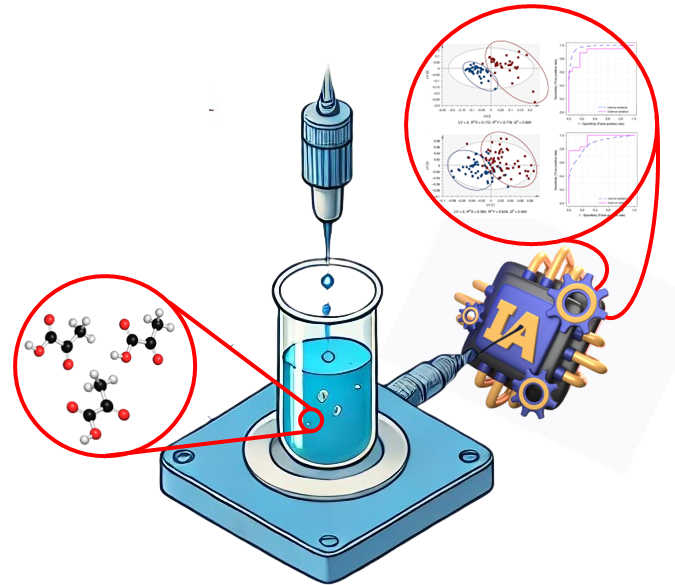
\includegraphics[width=2.5in]{figures/fig0.png}%
\end{wrapfigure}%
\begin{abstract}
Complementary Split Ring Resonators (CSRRs) have been extensively studied as planar sensors in the last two decades. However, their practical use beyond controlled environments remains limited due to reliance on high-end Vector Network Analyzers (VNAs), highly repeatable laboratory conditions, and special sample holders.

This work presents a novel approach to enhance the applicability of CSRR sensors in biomedical research through Machine Learning (ML) algorithms. A low-cost, benchtop CSRR-based system is proposed to quantify ethanol concentration in water solutions. ML-based analysis outperforms conventional statistical methods reported in the literature, improving accuracy and robustness. 

Ethanol samples from $10\%$ to $96\%$ concentration were prepared in commercial vials, generating 500 randomized measurements — a dataset significantly larger than typical studies. Principal Component Analysis (PCA) was employed for data exploration, while a Partial Least Squares Regressor (PLSR) trained with Leave-One-Group-Out Cross-Validation achieved a Root Mean Square Error in Prediction (RMSEP) of $3.7\%$ and a Limit of Agreement around $15\%$ within a $95\%$ Confidence Interval. No evidence of underfitting or overfitting was observed.

These results demonstrate the potential of CSRR-based sensors combined with ML techniques for quantifying bi-component liquid mixtures under realistic, uncontrolled conditions — paving the way for their application in biomedical scenarios.			   
\end{abstract} 

\begin{IEEEkeywords}
CSRR Sensors, Machine Learning, RF Biomedical, Resonators.
\end{IEEEkeywords}
\end{minipage}}}
\maketitle
\section{Introduction}
\label{sec:intro}
\IEEEPARstart{C}{omplementary} Split Ring Resonators (CSRR) were introduced as metasurfaces and metamaterials~\cite{falcone2004, Baena2005}, originally designed for microwave stopband filters, transmission lines, and antennas~\cite{GGarcia2005, Bonache2006, Mandal2006, Gil2007, Velez2008, Zhang2009}. Their sharp filtering behavior and sensitivity to surface surroundings~\cite{Grzegorczyk2005, Stevanovic2006, Bonache2006} soon positioned them as sensors~\cite{Boybay2012}, particularly for measuring complex permittivity of materials~\cite{Song2013, Lee2014, Lee2014_2, Ansari2015, Standaert2017, Su2019}.

In recent years, CSRR sensors have gained prominence in biomedical applications, particularly for quantifying solute concentrations in solvents~\cite{Velez2018, Omer2021, Zhang2019}. Notable applications include glucose detection in aqueous solutions~\cite{Omer2021, Martinic2025}, alongside microfluidic device integration~\cite{Patel2022, Jiang2023, Liu2024, Zhang2024}. However, despite promising laboratory results, none of these studies have demonstrated the practical applicability of CSRR sensors in real biomedical laboratory conditions, where environmental uncertainties and uncontrolled factors are present.

Machine Learning (ML) algorithms might solve this situation. They have been increasingly applied to CSRR sensors in the last five years~\cite{Prakash2022, Harrison2020, Kazemi2022, Abdolrazzaghi2023}, primarily to fit models linking Scattering Parameter (S-Parameter) features to concentration of solute~\cite{Martinic2025}. Recently, Multivariate Analysis (MVA) has been briefly introduced to this purpose~\cite{Trovarello2024}. Despite these advances, the full potential of ML algorithms to mitigate noise and variability in CSRR-based measurements under realistic conditions has not yet been fully explored. Furthermore, the literature lacks studies involving large datasets and appropriate sampling techniques, which are essential to build robust and generalizable models.

In Biomedical laboratories, measurement device is usually a benchtop equipment, the environmental conditions are not controlled, and laboratory staff is not trained in Radiofrequency measurements. Therefore, this work proposes a portable, low-cost benchtop CSRR-based system prone to uncertainties from the sensor, the Vector Network Analyzer (VNA), and measurment rutine. ML algorithms, specifically Principal Component Analysis (PCA) and Partial Least Squares Regression (PLSR), are employed to enhance system performance. A large and comprehensive database (around $500$ repetitions of $10$ samples of $9$ different concentrations) was built to enable robust training with Leave-One-Group-Out Cross-Validation (LOGO-CV), yielding a quantification model. This approach demonstrates that ML algorithms can enable CSRR-based sensors to be deployed in biomedical applications outside strictly controlled environments.

The text is organized as follows: Section~\ref{sec:csrrbenchTop} describes the measurement system, including the CSRR sensor, VNA, sampling methodology, and ML workflow. Section~\ref{sec:csrrPerformance} presents data visualization, traditional CSRR performance modeling, PCA exploration, and PLSR training results. Section~\ref{sec:csrrEval} compares the system's performance with conventional curve fitting methods. Finally, Section~\ref{sec:conclusion} summarizes the findings and the potential of CSRR-based systems in biomedical applications.

\section{CSRR benchtop System}\label{sec:csrrbenchTop}
\subsection{System Block Diagram}\label{ssec:sysBlockD}

\begin{figure}[!ht]
	\centering
	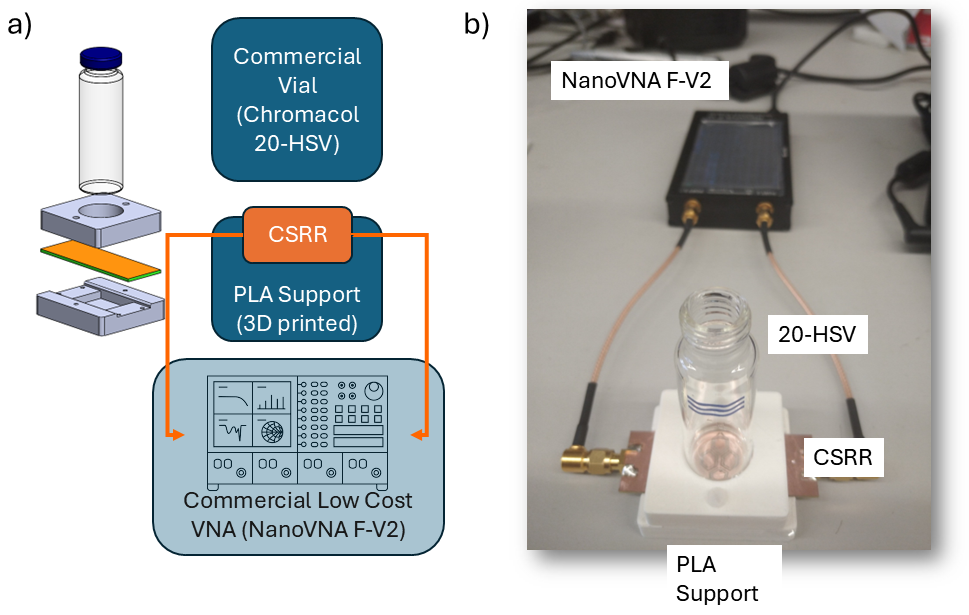
\includegraphics [trim = 0mm 0mm 0mm 0mm, clip, width=1\columnwidth]{figures/fig1.png}
	\caption{roposed benchtop CSRR system. (a) The commercial vial (Chromacol 20-HSV) containing the SUT is placed on the CSRR using a 3D-printed PLA support. The CSRR is connected to the low-cost VNA (NanoVNA F-V2) via two SMA cables. The NanoVNA operates either through its built-in graphical interface or via serial commands from a Python application running on a standard laptop. (b) Photograph of the real setup with a vial on top of the CSRR.}
	\label{fig:senBlockD}
	\vspace{-0.3cm}
\end{figure}

Figure~\ref{fig:senBlockD}(a) presents the block diagram of the CSRR-based system. Describing the measurement system is essential because, as discussed in Section\ref{sec:intro}, most studies optimize measurement setups to maximize sensor performance under controlled conditions.

In this contribution, the CSRR system is designed as a benchtop tool for biomedical laboratories. The Sample Under Test (SUT) is placed in a commercial vial (Chromacol 20-HSV) and positioned on the sensor using a 3D-printed PLA holder. This holder ensures the vial is consistently centered over the CSRR resonant structure, minimizing positional variability during measurements. 

Benchtop equipment must be compact, portable, and affordable to fit standard laboratory environments. The system measures the S$_{21}$ parameter, which some studies achieve through custom electronics~\cite{Omer2020, Omer2021}, while others rely on expensive commercial VNAs~\cite{Patel2022, Jiang2023, Liu2024}. Here, a low-cost commercial VNA (NanoVNA F-V2) was selected due to its affordability, performance in the $1$–$3$~GHz band, and compatibility with external laptops via serial commands.

he VNA is controlled by a custom GUI developed in Python, running on a commercial laptop. The GUI facilitates data acquisition, organizes data into structured databases, and enables continuous measurement. It also includes a quantification module to integrate trained ML models for real-time concentration predictions from S-parameter measurements. 
\subsection{CSRR Sensor}
\label{ssec:csrrSensor}

\begin{figure}[!t]
	\centering
	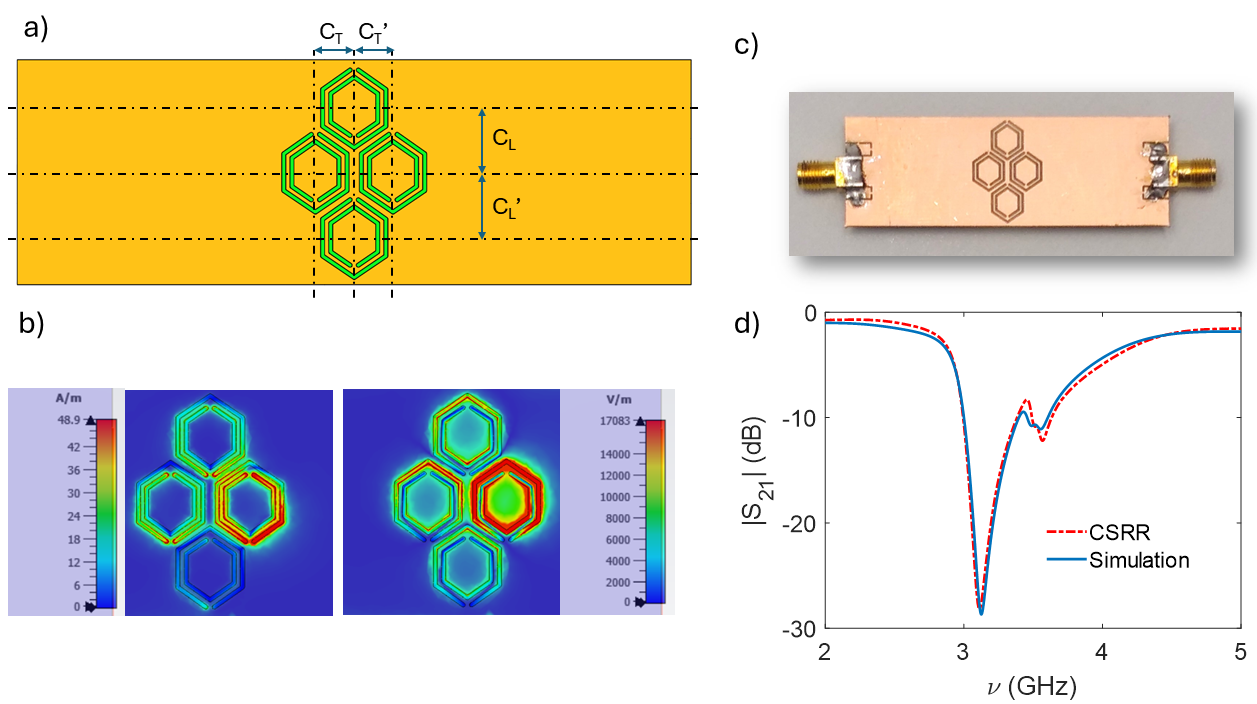
\includegraphics [trim = 0mm 0mm 0mm 0mm, clip, width=1\columnwidth]{figures/fig2.png}
	\caption{Modified CSRR. (a) Structure of the measured CSRR with asymmetrical honeycomb placement on a $22\times66$~mm PCB. The longitudinal honeycombs are positioned at $C_{L}=6.3$~mm and $C_{L}'=6.4$~mm from the PCB center, while the transverse honeycombs are placed at $C_{T}=3.7$mm and $C_{T}'=3.8$mm. (b) Simulated electric ($\vec{E}$\nicefrac{V}{m}) and magnetic field ($\vec{H}$\nicefrac{A}{m}) distributions on the honeycomb structure surface. (c) CSRR mounted with SMA connectors. (d) S$_{21}$ comparison between simulations and measurements with the CSRR unloaded (Keysight E5071C-240).}
	\label{fig:csrr}
	\vspace{-0.3cm}
\end{figure}

Figure~\ref{fig:csrr}(a) shows the structure of the CSRR used in this contribution, manufactured by Eurocircuits NV. The design is based on the honeycomb CSRR presented in\cite{Omer2020}, with modifications to modify its spectral response. Specifically, the vertical and horizontal symmetry was altered by $100$~$\mu$m, introducing an additional resonance around $3.5$~GHz close to the main resonance at $3.2$~GHz. This asymmetry intentionally degrades the measurement conditions by increasing the system's sensitivity to positional variations of the SUT. The coupling transmission line and the dimensions of each honeycomb are as defined in~\cite{Omer2020}, so the CSRR does not introduce further uncertainty in the measurement.

\subsection{Sampling Methodology}
\label{ssec:samplingMethod}

\begin{figure*}[!t]
	\centering
	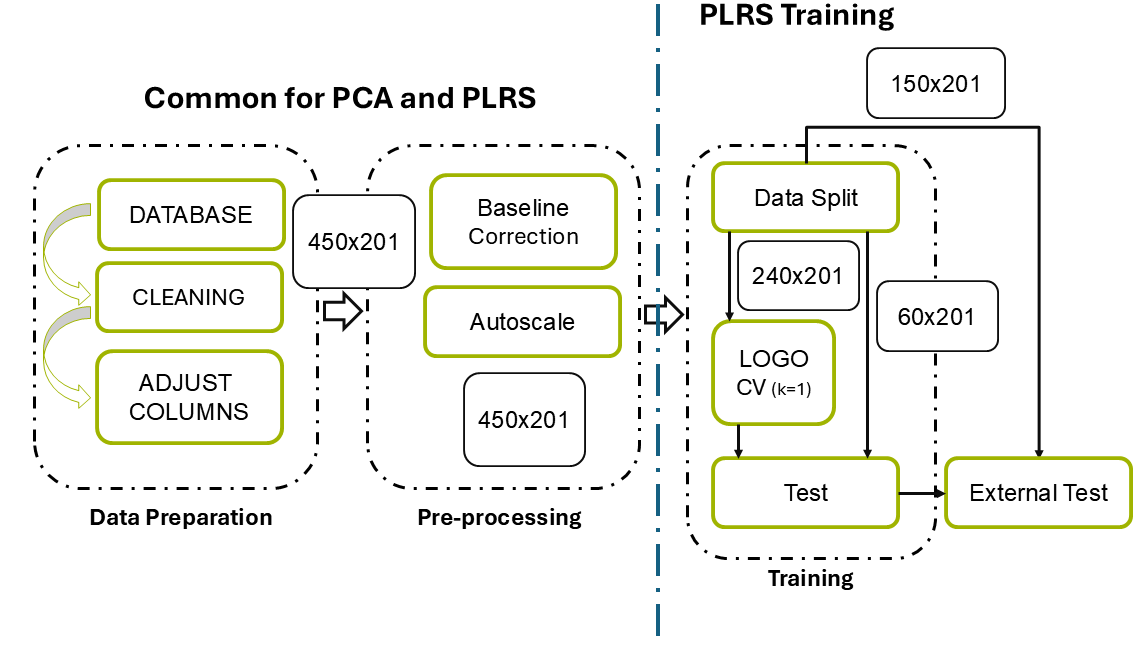
\includegraphics [trim = 0mm 0mm 0mm 0mm, clip, width=1.5\columnwidth]{figures/fig6_3.png}
	\caption{Block diagram of the developed workflow for training the bench-top CSRR system. In the Data Preparation step, the database is cleaned by extracting the actual data (features) from the metadata, resulting in a $450 \times 201$ feature matrix and a $5 \times 201$ baseline matrix. In the Pre-Processing step, the feature matrix baseline is corrected using the baseline matrix, applied to each round separately. In the Training step, the feature matrix is split into the training dataset ($300 \times 201$ matrix) and the test dataset ($150 \times 201$ matrix). These two steps are common to both PCA and PLSR training algorithms. The training dataset is then introduced into a leave-one-block-out cross-validation (LOGO-CV) scheme, which produces an optimized PLSR model. In the External Test step, the performance of the optimized model is evaluated by obtaining predictions from the test dataset.}
	\label{fig:workflow}
	\vspace{-0.3cm}
\end{figure*}

Sampling for training ML algorithms is a well-established field in Statistical Learning. The primary objective of any sampling technique is to randomize repetitions of each sample. This randomization mitigates undesired effects on the dataset, such as batch effects, repetition correlation, and instrumental error propagation~\cite{Wu2020}. 

In this study, samples were organized according to ethanol concentration in solution. The concentrations ranged from almost diluted ($10\%$ ethanol) to ethanol ($96\%$ purity), following the steps depicted in Figure~\ref{fig:avgData}(a). Badge solutions were prepared with the specified concentrations and poured into 10 commercial vials, randomly selected from a pool of 100 vials.

The 90 vials were labeled for randomization and identification, then stored together in a fridge at $5$~$^{\circ}$C for one day. The following day, the vials were removed and left at $23$~$^{\circ}$C (room temperature) for an hour. Five measurement rounds were performed, with the order of vials randomized in each round. Each round consisted of ten repetitions for each concentration, using different vials for each repetition, resulting in a total of $500$ measurements ($50$ measurements for each concentration). Before each round, the unloaded response of the CSRR sensor (S${21}$) was measured and used for baseline correction. 

In total, $500$ measurements were taken for baseline correction of the dataset, and training and testing of the ML model. Each measurement consisted of 201 data points recording $20\dot{\log\left(|S{21}|\right)}$ from $1.6$~GHz to $3$~GHz using the NanoVNA F-V2.
\subsection{Machine Learning Workflow}
\label{ssec:mlWorkflow}

As shown in figure~\ref{fig:workflow}, the workflow for the machine learning (ML) models used in this study consists of three main steps: data preprocessing, feature extraction, and model training. Initially, data is prepared and preprocessed to ensure consistency and quality. Next, dimensionality reduction techniques such as Principal Component Analysis (PCA) are applied to extract meaningful features. Finally, Partial Least Squares Regression (PLSR) is employed for model training and prediction. 
\subsubsection{Principal Component Analysis}
\label{sssec:pca}

Principal Component Analysis (PCA) was performed on the database generated as described in section~\ref{ssec:samplingMethod}. The dataset was prepared and pre-processed as shown in Figure~\ref{fig:workflow}, and PCA was carried out using the Statistics and Machine Learning Toolbox in MATLAB.

As shown in Figure~\ref{fig:workflow}, the dataset is cleaned by extracting metadata (labels, date of acquisition, etc.) and adjusting the number of features for each repetition, if necessary. The data matrix ($450 \times 201$) is then pre-processed in two steps. First, the baseline of each measurement round is corrected using the $20\dot{\log\left(|S_{21}|\right)}$ of the unloaded CSRR. Second, each $20\dot{\log\left(|S_{21}|\right)}$ is auto-scaled by calculating the mean, $\mu_{C}$, and standard deviation, $\sigma_{C}$, for each concentration in each round.

Up to 20 PCs were considered for the analysis. The explained variance (EV) of the dataset was calculated for each PC, and the cumulative EV was plotted (see figure~\ref{fig:pcaAnalysis}~(c)). The distribution of the repetitions in the reduced vector space was also plotted for the first three PCs.  

\subsubsection{Partial Least Squares Regressor}
\label{sssec:pls}

The results from the PCA analysis suggested that using all features in the $20\dot{\log\left(|S_{21}|\right)}$ spectrum could lead to good results in quantification. The most widely used predictor in this case is Partial Least Squares Regression (PLSR), which is especially suitable for datasets with a small number of repetitions per sample~\cite{Wold2001}.

Before starting the PLSR training, the feature matrix was pre-processed in the same way as for the PCA analysis (see Figure~\ref{fig:workflow}). The pre-processed data was then split into two subsets. Data from six concentrations was used for training (training dataset), while the remaining data was set aside for final testing (test dataset). Thus, the training dataset consisted of a $300 \times 201$ feature matrix, and the test dataset of a $150 \times 201$ matrix.

A Leave-One-Group-Out cross-validation (LOGO-CV) scheme was used for model training~\cite{Filzmoser2009}. This approach uses data from four rounds for training and reserves one round for validation, resulting in five evaluations of different PLSR models. The model with the best performance, in terms of Root Mean Square Error (RMSE), is then selected. The LOGO-CV scheme is run for different numbers of Latent Variables, up to $31$.

Once the PLSR model is trained, its evaluation is performed by introducing the test dataset and making predictions for the concentrations. In this case, predictions for $40\%$, $60\%$, and $80\%$ concentrations were calculated using the resulting model.

\section{CSRR System Performance}
\label{sec:csrrPerformance}
In this section, we present the results from the measurements, characterization of the frequency shift, and machine learning analysis of the CSRR system. The performance of the system is evaluated in terms of its ability to quantify the concentration of ethanol in water. We begin by discussing the traditional characterization of the system, followed by the PCA analysis of the dataset, and conclude with the evaluation of the PLSR model's performance.

\subsection{Acquired Database}
\label{ssec:mlMeasurement}
\begin{figure}[!t]
	\centering
	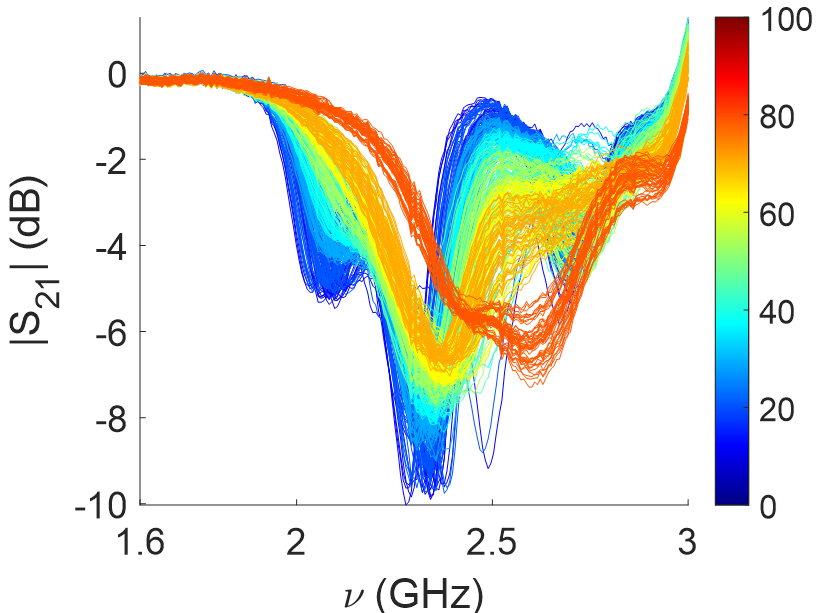
\includegraphics [trim = 0mm 0mm 0mm 0mm, clip, width=1\columnwidth]{figures/fig4_3.png}
	\caption{$20\dot{\log\left(|S_{21}|\right)}$ of each measurement in the generated dataset. Ethanol concentrations in clean water range from $10\%$ to $96\%$. Ten random commercial vials were selected for each concentration from a pool of $100$. Five rounds of measurements were performed, where in each round, the $20\dot{\log\left(|S_{21}|\right)}$ of the CSRR was recorded by placing a randomly selected vial on top of the sensor and continuing through the set of $90$ vials. Before each round, the $20\dot{\log\left(|S_{21}|\right)}$ of the unloaded CSRR was measured for baseline correction of the data.}
	\label{fig:mlMeasTaken}
	\vspace{-0.3cm}
\end{figure}

Figure~\ref{fig:mlMeasTaken} shows the $20\dot{\log\left(|S_{21}|\right)}$ of each measurement in the dataset used for ML model training and testing. Several features are evident upon visual inspection. First, a wide dispersion of the curves is observed for each concentration. Notably, the dispersion of the deepest resonance seems to decrease as the ethanol concentration increases.

Features around $2.1$~GHz and $2.5$~GHz show better discrimination between samples. Additionally, for $20\%$ ethanol, two repetitions exhibit an outlier behavior, with $20\dot{\log\left(|S_{21}|\right)}$ values deviating from the trend observed in the rest of the dataset.

Furthermore, outliers were identified for certain concentrations ($10\%$, $20\%$, and $40\%$) in rounds $1$, $2$, $3$, and $5$. The repetitions corresponding to $40\%$ ethanol showed one outlier in each round, likely due to a vial characteristic that differed significantly from the rest of the pool. However, the outliers for $10\%$ and $20\%$ ethanol appeared in different rounds, suggesting inconsistent handling of the vials during measurements.

\subsection{Frequency Shift Characterization}
\label{ssec:sysCharac}
\begin{figure}[!t]
	\centering
	\subfigure{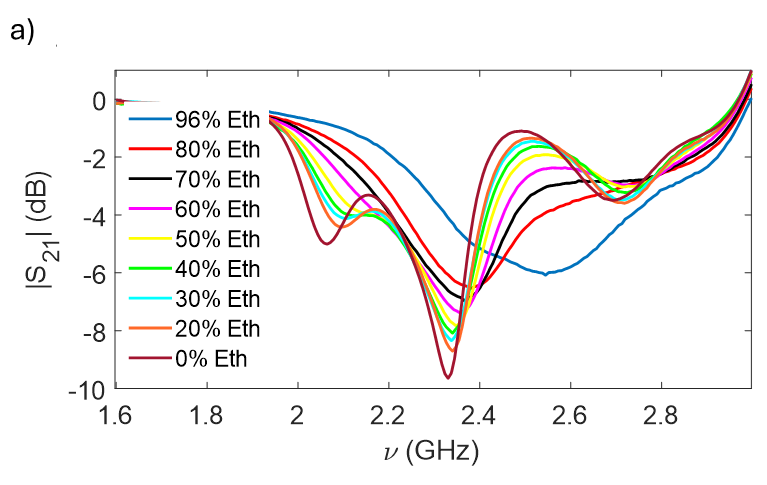
\includegraphics [trim = 0mm 0mm 0mm 0mm, clip, width=1\columnwidth]{figures/fig3_a.png}}
	\subfigure{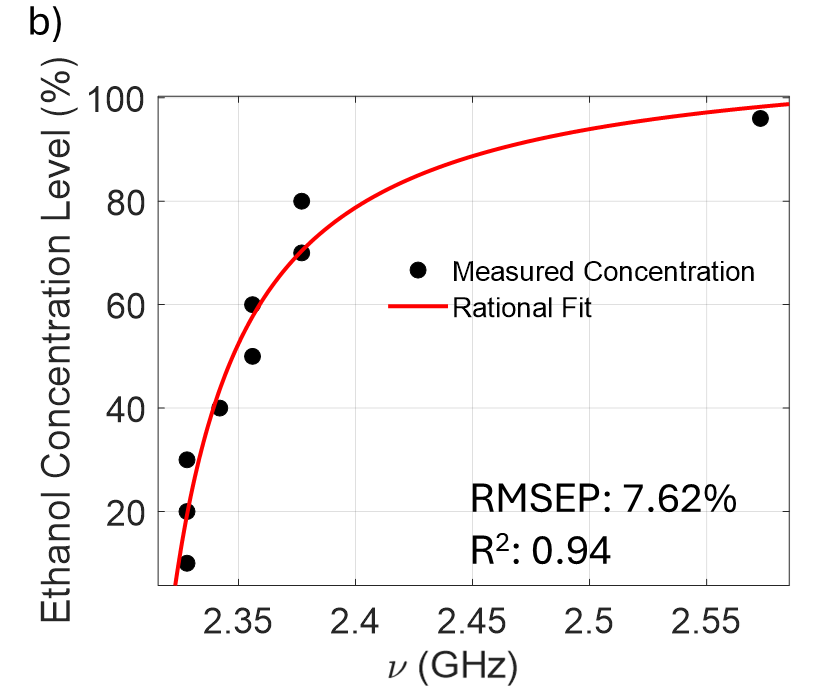
\includegraphics [trim = 0mm 0mm 0mm 0mm, clip, width=1\columnwidth]{figures/fig3_b.png}}
	%\hfill
	\caption{Traditional characterization of the CSRR system when measuring concentrations of ethanol diluted in clean water and poured in commercial vials. a) Averaged $20\dot{\log\left(|S_{21}|\right)}$ response of the generated database. b) Rational model for the frequency of the minimum observed in the averaged $20\dot{\log\left(|S_{21}|\right)}$ when every concentration of ethanol in clean water is observed ($10$, $20$, $30$, $40$, $50$, $60$, $70$, $80$, and $96$~$\%$)}
	\label{fig:avgData}
	\vspace{-0.3cm}
\end{figure}

Following studies presented in the literature, Figure~\ref{fig:avgData}(a) shows the averaged $20\dot{\log\left(|S_{21}|\right)}$ for each concentration. This plot illustrates how the shape of the S$_{21}$ parameter evolves with concentration, indicating a non-linear response of the system to ethanol. By evaluating the frequency shift of the most prominent resonance in Figure\ref{fig:avgData}(a)\cite{Abdolrazzaghi2023}, a rational fit of the deepest resonance yields the following expression:

\begin{equation}
	\label{eq:frequFitt}
	 C_{\%}(\nu) = \frac{p1\cdot\nu+p2}{\nu+q} 
\end{equation} 

where the frequency, $\nu$, is in GHz, $p1 = 110.7274$~$\nicefrac{\%}{GHz^{2}}$, $p2 = -257.0246$~$\nicefrac{\%}{GHz}$, and $q = -2.2893$~GHz. The $R^{2}$ of the fit is $0.9422$ and the RMSE is $7.9208$~$\%$. The fitting was performed using the Curve Fitting Toolbox from MATLAB. This model is shown in Figure~\ref{fig:avgData}~(b).

\subsection{Principal Component Analysis}
\label{ssec:pcaAnalysis}

\begin{figure}[!t]
	\centering
	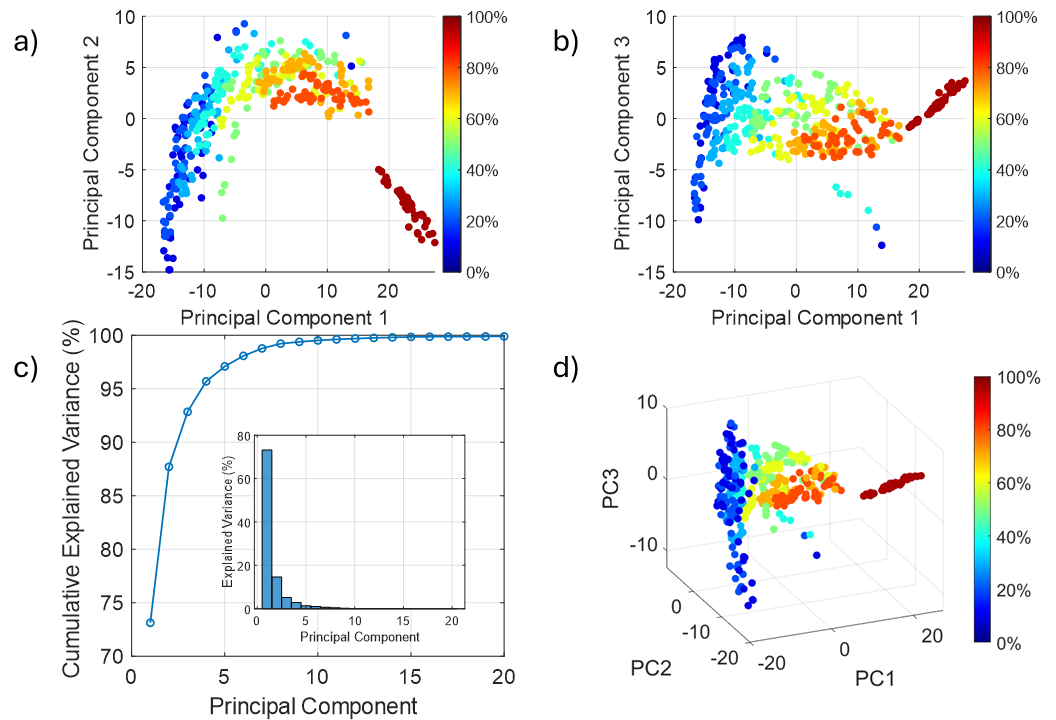
\includegraphics [trim = 0mm 0mm 0mm 0mm, clip, width=1\columnwidth]{figures/fig5_3.png}
	\caption{Principal Component Analysis (PCA) of the dataset generated as described in section~\ref{ssec:samplingMethod}. a) Distribution of each repetition in the reduced vectorial space when representing the second Principal Component (PC) with respect to the first PC. b) Distribution of each repetition in the reduced vectorial space when representing the third Principal Component (PC) with respect to the first PC. c) Cumulative Explained Variance of the dataset (in $\%$) with respect to the considered PCs and Explained Variance distribution over the set of PCs considered. d) 3D distribution of each repetition in the reduced vectorial space.}
	\label{fig:pcaAnalysis}
	\vspace{-0.3cm}
\end{figure}

Figures~\ref{fig:pcaAnalysis}~(a), (b), and (d) show the distribution of the repetitions in the reduced vector space of the extracted PCs. In all figures, the first PC dominates, which can be associated with the ethanol concentration in the solution. The spread in this component indicates that, despite the careful preparation of each stock solution, the system is sensitive enough to detect relatively small variations in concentration.

As shown in Figure~\ref{fig:pcaAnalysis}~(c), $95\%$ of the Explained Variance (EV) is contained within the first three Principal Components (PCs). Most of this variance is concentrated in the first PC ($73\%$), while the remaining components account for less than $15\%$ of the EV.

Additionally, these figures show a spread in the second and third components, which can be attributed to variability introduced by the commercial vials and the measurement process itself (see Figure~\ref{fig:pcaAnalysis}(d)). It is this variability where the outliers are observed. Specifically, the plot in Figure~\ref{fig:pcaAnalysis}(b) helps identify the outliers at $0\%$, $20\%$, and $40\%$ concentrations, as shown in Figure~\ref{fig:mlMeasTaken}.   

\subsection{Partial Least Squares Regressor Training}
\label{ssec:plsRegressor}

Once the workflow presented in Figure~\ref{fig:workflow} is completed, several intermediate results provide insights into the performance of the obtained model. Figure~\ref{fig:plsrStatistics}~(a) shows the evolution of the Root Mean Square Error (RMSE) with respect to the number of components used in the PLSR during the LOGO-CV scheme iterations. It can be observed that with 6 Latent Variables (LVs), the MSE of the best model from the $5$ generated by the LOGO-CV scheme is minimized to approximately $6.8$, resulting in a Root Mean Square Error in Cross Validation (RMSECV) of approximately $\sim3.62\%$.

Additionally, the most important features in the training dataset were identified using the Variable Importance in Projection (VIP) scores for each feature~\cite{Chong2005}. The calculated scores provide information on the average importance of each feature in the projection of the repetitions onto the reduced vector space handled by the PLSR.

This information can be used to trim the feature matrix to focus on the most relevant part of the $20\dot{\log\left(|S_{21}|\right)}$. There are various ways to define the threshold for determining which features are more important than others~\cite{Ansari2015}. However, a commonly used approach is to consider features with a mean VIP score greater than 1 as relevant.

\begin{figure}[!t]
	\centering
	\subfigure{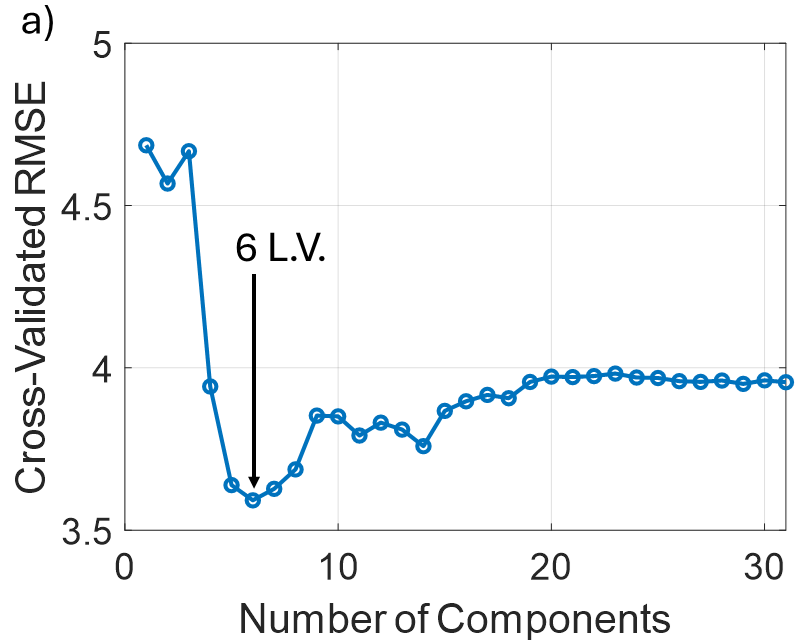
\includegraphics [trim = 0mm 0mm 0mm 0mm, clip, width=1\columnwidth]{figures/fig7_a.png}}
	\subfigure{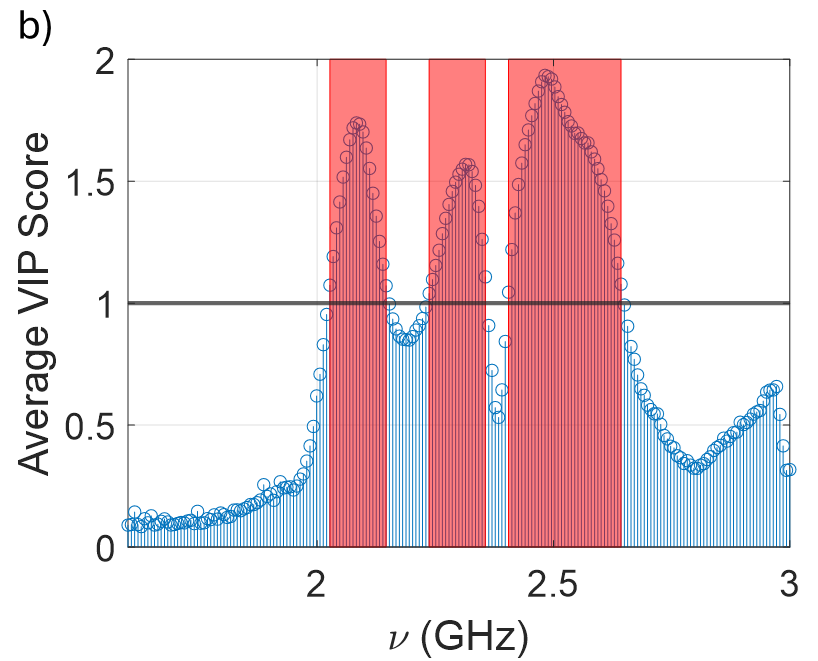
\includegraphics [trim = 0mm 0mm 0mm 0mm, clip, width=1\columnwidth]{figures/fig7_b.png}}
	%\hfill
	\caption{Statistics of the Partial Least Squares Regressor (PLSR) trained with the generated dataset: a) Evolution of the Mean Squared Error (MSE) with the number of Latent Variables (LVs) during the Leave-One-Block-Out Cross-Validation (LOGO-CV). b) Mean Variable Importance in Projection (VIP) scores for each feature from 1.6GHz to 3GHz, with scores greater than 1 highlighted in pink (\squarecolor[pink]).}
	\vspace{-0.3cm}
	\label{fig:plsrStatistics}
\end{figure}

Figure~\ref{fig:plsrStatistics}(b) shows the VIP scores for the training dataset after optimizing the PLSR to 6 LVs. In this figure, pink areas (\squarecolor[pink]) highlight scores greater than 1. It can be observed that the most important parts of the $20\dot{\log\left(|S_{21}|\right)}$ correspond to data around $2.1$~GHz, $2.45$~GHz, and $2.5$~GHz. These frequency ranges align with the most significant differences between concentrations observed in Figure~\ref{fig:mlMeasTaken}.

\subsubsection{Performance in Cross Validation}
\label{sssec:perfCV}

\begin{figure}[!t]
	\centering
	\subfigure{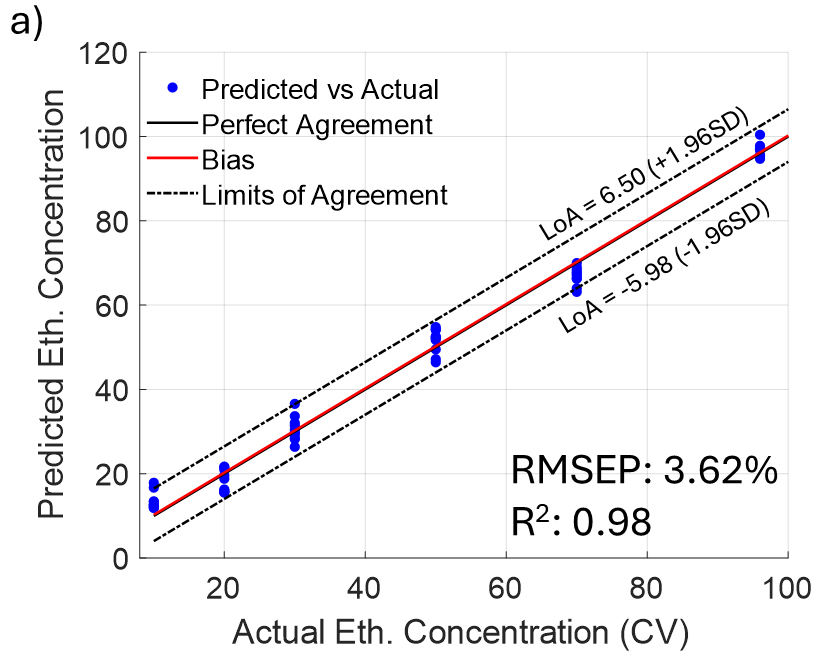
\includegraphics [trim = 0mm 0mm 0mm 0mm, clip, width=1\columnwidth]{figures/fig8_a.png}}
	\subfigure{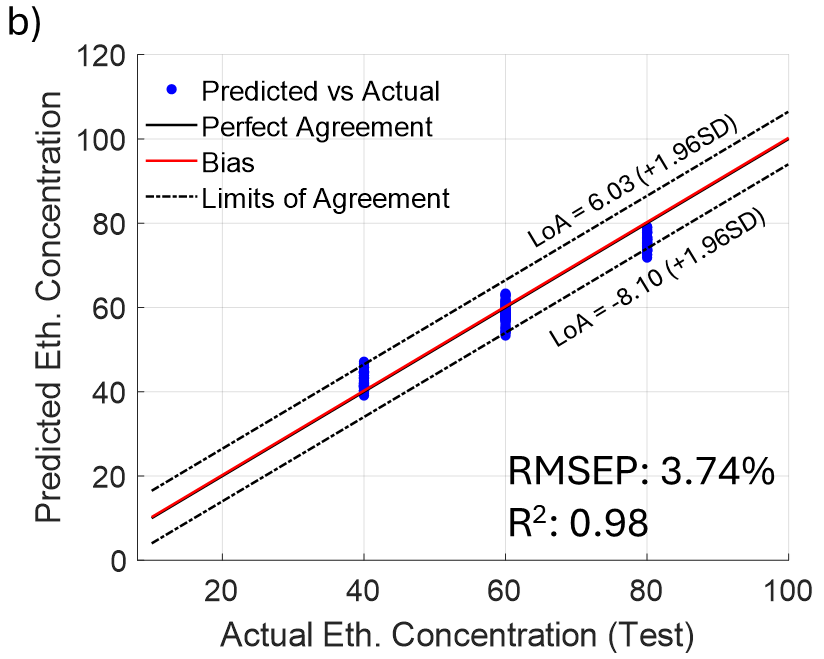
\includegraphics [trim = 0mm 0mm 0mm 0mm, clip, width=1\columnwidth]{figures/fig8_b.png}}
	%\hfill
	\caption{Summary of the PLSR performance. The plots include Predicted versus actual ethanol concentration in $\%$, the ideal perfect concentration, the bias introduced by the model and the upper and lower LoAs at $95\%$ CI. a) Predictions obtained during the Leave-One-Block-Out Cross-Validation (LOGO-CV) for the training dataset. b) Predictions obtained for the test dataset.}
	\vspace{-0.3cm}
	\label{fig:plsrResults}
\end{figure}

As mentioned in section~\ref{ssec:plsRegressor}, the LOGO-CV training scheme generates five PLSR models per set of Latent Variables (LVs). The model with the lowest Root Mean Square Error (RMSE) is selected as the best representative for the LV set.

According to Figure~\ref{fig:plsrStatistics}~(a), the PLSR model with six LVs provides the best performance during the LOGO-CV. This model was then used to make predictions on the training dataset, where repetitions for $20\%$, $30\%$, $50\%$, $70\%$, and $96\%$ concentrations were included in the training set, while $20\%$ of these repetitions were set aside for evaluation.

Figure~\ref{fig:plsrResults}~(a) shows the PLSR predictions for the repetitions kept aside. The RMSE in cross-validation (RMSECV) was around $3.62\%$, with an $R^{2}$ of $0.98$. The Limits of Agreement (LoA), calculated using the Bland-Altman method for the $95\%$ confidence interval, resulted in a $13.5\%$ deviation from linear prediction.
 
\subsubsection{Performance in Test}
\label{sssec:perfTest}

Despite the test during training is performed with repetitions that the LOGO-CV scheme had no access to, it is interesting to test if the PLSR model is able to predict concentrations that the training process have not seen before. 

In section~\ref{ssec:mlWorkflow}, the database was divided into training dataset and test dataset. The test dataset contained the repetitions of $40\%$, $60\%$ and $80\%$ samples. This dataset was used to obtain predictions with the PLSR model and evaluate its performance against "blind" samples.

Figure~\ref{fig:plsrResults}~(b) shows the predictions obtained for the test dataset. These predictions produced a RMSE in Prediction (RMSEP) about $3.7$~$\%$, very close to the RMSECV, with a R$^{2}$ coefficient of $0.98$. The LoAs were calculated in the same way presented in previous section, resulting in a LoA~$\sim14.2\%$ with a $95\%$ of Confident Interval. The PLSR models showed a $1.5\%$ bias when predicting the concentrations of the test dataset and the LoAs increased also $\sim1\%$ with respect to the LoAs obtained in traini

\section{CSRR System Evaluation}
\label{sec:csrrEval}

In this study, we demonstrate the impact of applying ML algorithms in measuring liquid concentrations with a CSRR-based bench-top system. When properly applied, ML techniques not only reveal the properties of the generated datasets but also enhance the performance of low-cost bench-top systems for predicting concentrations of substances under test (SUTs) when measurement conditions are very close to a real biomedical application.

For a bench-top system like the presented in section~\ref{sec:csrrbenchTop} the measurement procedure and the commercial vials used regularly in laboratories, introduce a considerable the most observable variability across repetitions. In the literature, this variability is managed, either enhancing the hardware of the system, which might be impossible in many of the cases due to the increase in hardware cost, or designing ad-hoc solutions that reduce variability, as it happens with the vials.

Furthermore, the inefficiency of using one-dimensional analysis, such as frequency shift, has been demonstrated in this study. Section~\ref{ssec:sysCharac} highlights how a large and robust dataset (acquired as explained in section~\ref{ssec:mlMeasurement}) reveals significant variability and large standard deviations across repetitions, making it clear that simple curve fitting is unlikely to accurately predict the concentration of the SUT. 

In particular, in this study, the combination of the presented system, measurement procedure, and commercial vials resulted in a curve-fitting model based on the frequency shift of the S$_{21}$ parameter with ethanol concentration, yielding an RMSE of $7.62$~$\%$. This performance is clearly insufficient for biomedical applications. Therefore, for systems intended for biomedical or laboratory use as benchtop devices, multivariate analysis is essential to improve both accuracy and robustness.

The proposed workflow with an intensive, coherent and properly randomized sampling procedure, a preliminar exploration of the dataset and a full training of a multivariate quantification model have demonstrated their boosting capabilities.

A preliminay exploration of the obtained datasets, as explained in section~\ref{ssec:pcaAnalysis}, lead to a better understanding of the behaviour of CSRR bench-top systems. It also orientate to the proper prediction model useful for the application and the final use.

In particular, for the benchmark problem of ethanol concentration diluted in clean water, the PCA shows the variability of the dataset concentrated around 4 Principal Components (PCs), as it is shown in figure~\ref{fig:pcaAnalysis}. The first PC is clearly related to the ethanol concentration in the solution, while the rest of the PCs might be related to the variability introduced by the commercial vials and the measurement procedure. In accordance with this, the training evolution of the PLSR model showed that 6 LVs minimized the RMSECV (see figure~\ref{fig:plsrStatistics}~(ã)). Also, the VIP scores analysis confirmed the multivariate nature of the problem (see figure~\ref{fig:plsrStatistics}~(b)).
 
In fact, the trained PLSR model trained with the workflow presented in section~\ref{ssec:mlWorkflow}, shows a better performance than the univariate model. In particular, a reduction by a factor of $\sim2$ in the RMSE at test (RMSEP $=3.74$~$\%$). Also, the LoAs are stable over the range of concentrations considered in the test dataset and very similar at training and test. This behaviour in training and test shows the robustness of the PLSR model compared with the quantification models presented in the literature. 

\section{Conclusions}
\label{sec:conclusion}
As a result of the presented study, it has been demonstrated that the performance of low-cost, benchtop devices, ready to be used in laboratory settings, can be significantly enhanced by applying Machine Learning algorithms, techniques, and workflows. This demonstration was carried out using a representative example of the benchmark problem of quantifying ethanol concentration diluted in clean water. The results show that an extensive sampling campaign, coupled with the use of ML algorithms—specifically PCA and PLSR—can improve the performance of traditional curve fitting by a factor of 2.

These results overcome the limitations associated with univariate analysis of the S$_{21}$ parameter in CSRR-based systems, particularly when applied to real-world scenarios such as biomedical laboratories. This opens up the opportunity to utilize CSRR-based systems as benchtop devices in biomedical applications, advancing their development as valuable tools for screening, diagnosis, and monitoring.

\section*{Acknowledgment}
Author want to thank Professor Antonio Pardo and Gema Guedes, Ph.D. for their collaboration during experiments in the laboratory and their understanding on the increasing entropy inside it.

\bibliographystyle{IEEEtran}
\bibliography{bib/ieeeBibCSRRandML}
%\vspace{-1cm}
\vskip -2\baselineskip plus -1fil

\begin{IEEEbiography}[{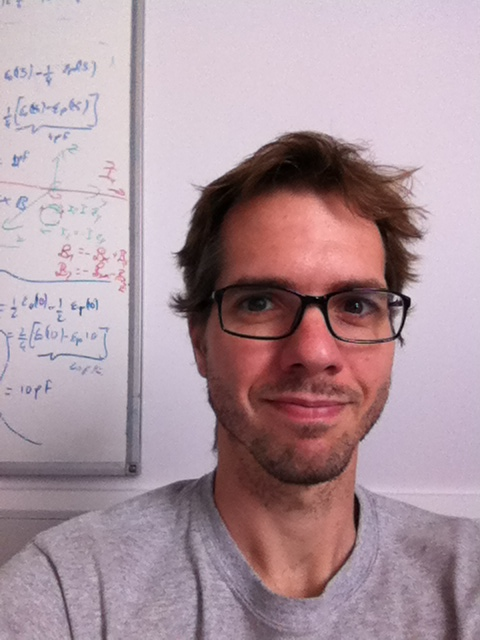
\includegraphics[width=1in,height=1.25in,clip,keepaspectratio]{figures/JAV-Website-Photo.jpg}}]{Javier Alonso-Valdesueiro}
was born in Madrid, Spain, in 1980. He earned a Telecommunications Engineering degree from the University of Alcalá, Madrid, in 2006, and a Ph.D. from the Polytechnic University of Catalonia, Barcelona, in 2011. From 2012 to 2020, he worked on developing electronic instrumentation for NMR experiments, initially at the C.E.A Center in France, followed by the University of Southampton in the UK, and later as a Marie Skłodowska-Curie Fellow at the University of the Basque Country (UPV/EHU). Over the past four years, he has advanced his career as an RF and instrumentation engineer in both private companies and public research centers, including TECNALIA Innovation Foundation and the Institute of Biomedical Engineering of Catalonia. Recently, he was appointed Assistant Professor in the Department of Electronic and Biomedical Engineering at the University of Barcelona. His current research focuses on radio-frequency (RF) devices for MRI, instrumentation electronics for gas sensing applications, and advancements in RF sensor technologies.
\end{IEEEbiography}
\vskip -2\baselineskip plus -1fil
%\vspace{-1.5cm}
\end{document}
